\chapter{Conceptos base}

Es relevante hacer una introducción a los conceptos y herramientas que se utilizan en el desarrollo del informe para poder hacer de este trabajo algo más autocontenido. Además en la sección de estado del arte se exploran las soluciones existentes para conectar un simulador de vuelo a un autopiloto.

Este capítulo fue escrito a medida que se avanzó en el proyecto para poder entrar más en detalle en conceptos técnicos que de otra forma serian omitidos.

\section{Marco teórico}

\subsection{Repositorios en GitHub}

GitHub \cite{github} es una plataforma que permite a sus usuarios mantener repositorios de código fuente creados con el software ``git'' \cite{git}, el programa de control de versiones más popular a día de hoy. Un repositorio es un espacio en el que se guarda cada archivo del código fuente de un programa junto con todas las versiones anteriores que se vayan produciendo a medida que este se desarrolla, como un historial. Algunas de las funciones que habilitan los repositorios en línea son permitir al programador mantener una copia del software en el que esté trabajando (evitando que una perdida de datos en el equipo local sea catastrófica). Facilitar el trabajo colaborativo entre varios programadores que suben los cambios al mismo repositorio. Llevar un registro de versiones anteriores del programa a los que por alguna razón se quiera volver (quizá para resolver un bug o regresiones), entre otros.

Al día de hoy todos los proyectos con cierto grado de complejidad son hospedados en un repositorio, sea en línea con GitHub, alguna de las alternativas o localmente. La ventaja de utilizar software de control de versiones es significativa e incluso una necesidad si el proyecto es muy complejo. Todo el código que sea escrito durante el proyecto será registrado en un repositorio al cual se le agregará documentación para facilitar la aplicación que este tenga, de forma que se pueda aprovechar sin necesidad de leer este informe. Además si se continúa trabajando en el software cualquier cambio se verá reflejado en línea.

\subsection{Arquitectura de ArduPilot}

ArduPilot es un software autopiloto que puede administrar el movimiento de una gran variedad de vehículos como drones, aviones de ala fija, autos o submarinos. Un usuario convencional instala un hardware autopiloto como Pixhawk en el vehículo y luego por medio de antenas para la comunicación por radio y de transmisión de telemetría controla el vehículo, además de monitorear su estado en alguno de los software de estación en tierra como Mission Planner.

Internamente, la función de ArduPilot es definir la intención de lo que está intentando hacer el piloto interpretando las lecturas del radiocontrol, convertir esto en un objetivo de control de actitud con valores de roll, pitch y yaw si es una aeronave y de posición si se tiene un plan de vuelo cargado. Estimar la actitud y posición actual por medio de los sensores internos y externos del autopiloto. Para finalmente generar una acción de control que permita a la aeronave alcanzar su objetivo desde su estado actual.

Todo este proceso y las demás características de ArduPilot están escritas en C++ y el código fuente actualizado está disponible en GitHub \cite{ap-github-repo}. En el contexto de código el programa principal que carga ArduPilot es el del vehículo, para cada tipo de vehículo se tiene una clase principal llamada ArduCopter, ArduPlane, ArduRover, etc. Esto es así porque permite reducir la cantidad de código que se deba cargar al autopiloto, los primeros hardware autopiloto tenían una capacidad de memoria de solo lectura muy limitada. El programa específico del tipo de vehículo procede a cargar todas las librerías que vaya a necesitar, estas librerías son comunes para todos los tipos de vehículo y se tiene la opción de incluir o eliminar cada una de la compilación final. Las librerías más importantes son los drivers para interactuar con sensores, modelos de estimación de actitud por filtro de Kalman, conversión de valores de radiocontrol a salidas de servo PWM, entre otras.

Esta arquitectura modular que tiene ArduPilot es conveniente para el proyecto, ya que se tiene una base si lo que se intenta lograr es algo similar a lo que ya está programado.

\subsection{X-Plane SDK}

Laminar Research, el desarrollador del simulador de aeronaves X-Plane ofrece un kit de librerías para el desarrollo de plug-ins muy completo \cite{xplane-sdk}. La librería está diseñada para ser enlazada a proyectos escritos en C++ estableciendo en el compilador la ubicación de los archivos ``header'' para tener una descripción de las funciones disponibles en el editor y la ubicación de una versión compilada de la librería. La SDK es muy completa permitiendo hacer cualquier cosa con la simulación, si se tiene experiencia en desarrollo de videojuegos las funciones que entregan las librerías serán familiares.

Los plug-ins para el simulador de vuelo son fundamentales para muchos usuarios, las cabinas realistas con instrumentación física y otras características inmersivas se sostienen sobre plug-ins para comunicarse con hardware externo. Existen además plug-ins de venta comercial que agregan funciones que Laminar Research quizá no tiene intención de agregar pues está fuera del alcance de X-Plane, pero que algunos usuarios están dispuestos a pagar por su función.

La SDK se puede configurar al momento de la compilación para establecer la versión mínima de X-Plane para la que se quiere exportar el plug-in, las versiones nuevas de X-Plane son retrocompatibles con plug-ins creados para versiones anteriores. Naturalmente, si se desea hacer uso de una función introducida en las versiones más actuales el plug-in no podrá funcionar en los X-Plane antiguos. En la documentación de la SDK está bien definida en que versión se introdujo cada función.

Otra consideración es que X-Plane 9, el simulador utilizado actualmente en el laboratorio de técnicas aeroespaciales, es exclusivamente de 32-bit. Y las versiones de X-Plane desde la 10 son de 64-bit. Para el desarrollo de plug-ins se debe definir la arquitectura de bits al momento de compilar, por lo que si se quiere crear un plug-in compatible con la mayor cantidad de versiones posible se debe definir una versión de X-Plane antigua, y compilar para 32 y 64 bits.

\section{Estado del arte}

\subsection{Simulación conectada a ArduPilot}

ArduPilot está programado para ser compatible con una amplia variedad de microcontroladores. Una consecuencia de esto es que también se puede compilar para ser ejecutado en un computador convencional, de manera paralela con un simulador de vuelo \cite{ardupilot-sitl}. Esto ha llevado al desarrollo de una versión de ArduPilot dedicada para realizar pruebas con la técnica ``Software-in-the-Loop'', con toda la infraestructura siendo ejecutada en el mismo computador.

\begin{figure}[h]
    \centering
    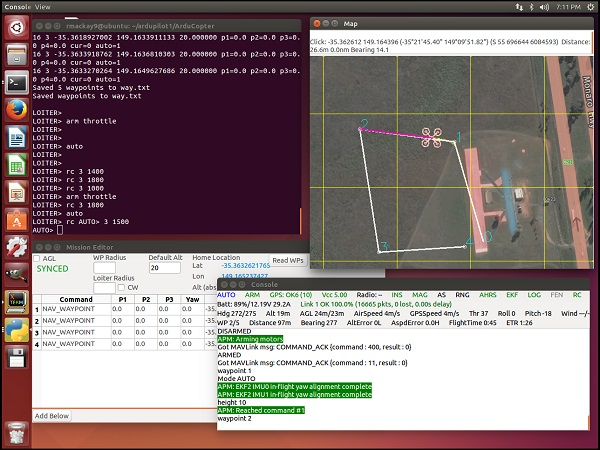
\includegraphics[width=0.7\textwidth]{sitl.jpg}
    \caption[ArduPilot ejecutando pruebas SITL.]{ArduPilot ejecutando pruebas SITL.\footnotemark}
    \label{fig:sitl}
\end{figure}
\footnotetext{\url{https://ardupilot.org/dev/docs/sitl-simulator-software-in-the-loop.html}}

Una limitación importante de esta solución es que el código no está corriendo en un autopiloto, por lo que se hace más complicado validar que los cambios que se hagan a ArduPilot funcionarían en uno. Para resolver este problema se ofrece de manera alternativa ejecutar una simulación (menos fiel a la realidad) dentro del mismo autopiloto \cite{sim-on-hardware}. Pero esto se ve evidentemente limitado por la capacidad de procesamiento del hardware autopiloto, el que se ve estresado por estar corriendo una simulación completa por sobre la programación convencional, además no ofrece una visualización en tiempo real además de la telemetría de Mission Planner.

\subsection{Hardware-in-the-Loop en PX4}

El software autopiloto PX4 ofrece un modo de simulación para realizar pruebas ``Hardware-in-the-Loop'' que es desarrollado por la comunidad \cite{px4-hitl}. Esta función está integrada en el firmware sin necesidad de hacer grandes cambios, en el programa de estación en tierra QGroundControl se debe activar la opción ``HITL'' y establecer algunos parámetros.

\begin{figure}[h]
    \centering
    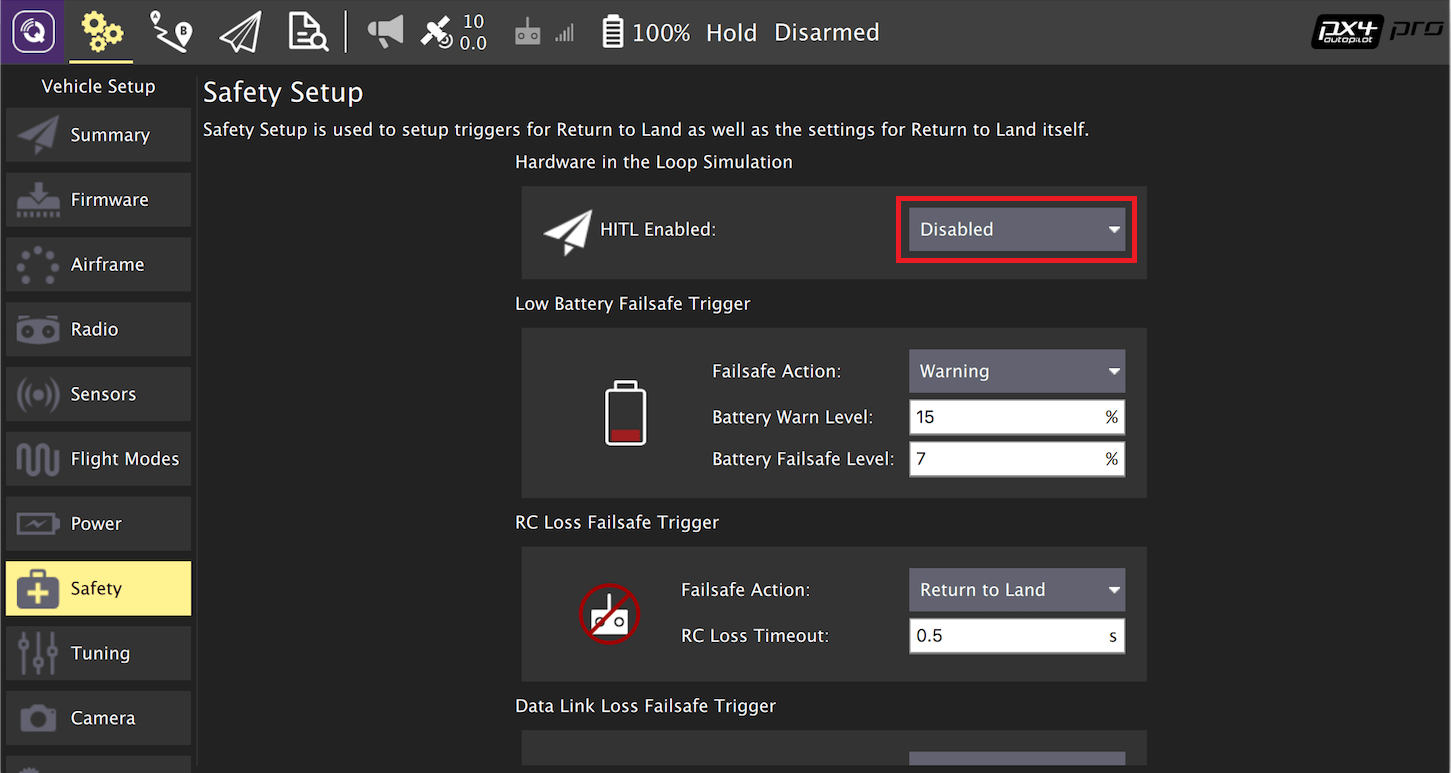
\includegraphics[width=0.7\textwidth]{px4-hitl.png}
    \caption[Configurando modo HITL en QGroundControl.]{Configurando modo HITL en QGroundControl.\footnotemark}
    \label{fig:px4-hitl}
\end{figure}
\footnotetext{\url{https://docs.px4.io/main/en/simulation/hitl.html}}

Según la documentación de esta función, el modo HITL es compatible con los simuladores ``FlightGear'', ``JSBSim'' y ``AirSim'', además de ofrecer la misma opción de ArduPilot de ejecutar una simulación simplificada en el mismo autopiloto en paralelo con el programa normal.